\subsection{Determinante}
    \begin{definition}{Determinante}\\
        Die Determinante gibt an, ob eine Matrix invertierbar ist.
        \begin{equation*}
            \det(A)
            \left\{
                \begin{array}{lll}
                    \neq 0   &\Rightarrow    & A^{-1} \text{ existiert. }\\
                    = 0     &\Rightarrow    & A^{-1} \text{ existiert nicht. }
                \end{array}
            \right.
        \end{equation*}
    \end{definition}

    \begin{theorem}{Eigenschaften von Determinanten}
        Gegeben zweier \textit{quadratischer Matrizen} $A$, $B$ 
        sowie einer \textit{quadratischen Dreiecksmatrix} $D$.
        \begin{align*}
            &\det(E)        &&=1                     \\
            &\det(D)        &&=\prod_{i=1}^n d_{ii}  \\
            &\det(A\cdot B) &&=\det(A)\cdot\det(B)   \\
            &\det(A^T)      &&=\det(A)               \\
            &\det(A^{-1})   &&=\frac{1}{\det(A)}     \\
            &\det(m\cdot A) &&=m^n\cdot\det(A)\, \text{ mit } m\in \R
        \end{align*}
    \end{theorem}

    \begin{theorem}{Geometrische bedeutung der Determinante}


        \begin{wrapfigure}[16]{hr!}{0.35\linewidth}
            \vspace{-10pt}
            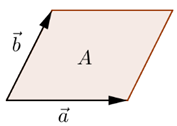
\includegraphics[width=0.9\linewidth]{images/det-vis-2d.png}
            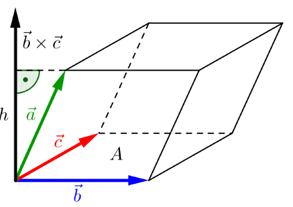
\includegraphics[width=0.9\linewidth]{images/det-vis-3d.png}
        \end{wrapfigure}
        Die Spalten einer $2\times 2$-Matrix $A$ spannen ein Parallelogram auf.
        Die Determinante der Matrix $A$ ist dabei gerade der \textbf{Flächeninhalt} des aufgespannte Parallelogram.
        \vspace{1.25em}

        Werden Spalten einer $3\times 3$-Matrix $B$ als raum Vektoren betrachtet, 
        spannen diese einen Spat auf.
        Die Determinante der Matrix $A$ ist dabei gerade das $Volumen$ des aufgespannten Spat.
        \vspace{1em}
    \end{theorem}

    \begin{formula}{Determinante einer $1\times 1$-Matrix}
        \begin{equation*}
            \det(A)=A_{11}
        \end{equation*}
    \end{formula}

    \begin{formula}{Determinante einer $2\times 2$-Matrix}
        \begin{equation*}
            \det(A)=\abs{A}=a\cdot d-b\cdot c
        \end{equation*}
    \end{formula}

    \begin{formula}{Determinante einer $3\times 3$-Matrix}\\
        \begin{wrapfigure}{r}{0.4\linewidth}
            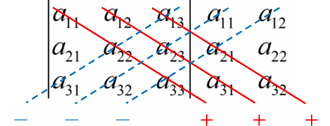
\includegraphics[width=0.9\linewidth]{images/det3x3.png}
        \end{wrapfigure}
        Die Formel für die Berechnung der Determinante einer $3\times 3$-Matrix ist rechts Gegeben.

        \begin{align*}
            \det(A)&=\abs{A}\\
            &= a_{11}\cdot a_{22}\cdot a_{33} 
            + a_{12}\cdot a_{23}\cdot a_{31} 
            + a_{13}\cdot a_{21}\cdot a_{32}\\
            &- a_{13}\cdot a_{22}\cdot a_{31} 
            - a_{11}\cdot a_{23}\cdot a_{32} 
            - a_{12}\cdot a_{21}\cdot a_{33} 
        \end{align*}
    \end{formula}

    \begin{formula}{Determinante einer $n\times n$-Matrix nach Laplace}\\
        Gegeben einer $n\times n$-Matrix $A$, 
        wird zum berechnen der Determinante eine feste Zeile $i$ oder Spalte $j$ gewählt,
        nachder die Determinante entwickelt wird.

        \textbf{Entwicklung nach Zeile}
        \[\det(A)=\sum_{j=1}^n{(-1)}^{i+j}\cdot A_{ij}\cdot\det(A_{ij})\]
        \textbf{Entwicklung nach Spalte}
        \[\det(A)=\sum_{i=1}^n{(-1)}^{i+j}\cdot A_{ij}\cdot\det(A_{ij})\]

        Bezeichnungen:
        \begin{itemize}
            \item $a_{ij}$ ist das Element der Matrix $A$ in der $i$-ten Zeile und $j$-ten Splate
            \item $A_{ij}$ ist die Matrix, die durch das Weglassen der $i$-ten Zeile und $j$-ten Spalte entsteht. 
        \end{itemize}

        \begin{highlight}{!}
            Um den Rechenaufwand zu minimieren, entwickelt man nach derjenigen Zeile oder Spalte, 
            in der die meisten Nullen stehen. 
        \end{highlight}
    \end{formula}
